The second model is a definition closer to the actual VGG implementation\footnote{\href{https://towardsdatascience.com/step-by-step-vgg16-implementation-in-keras-for-beginners-a833c686ae6c}{https://towardsdatascience.com/step-by-step-vgg16-implementation-in-keras-for-beginners-a833c686ae6c}}:
\begin{center}
    \begin{verbatim}
        Model: "sequential"
        _________________________________________________________________
        Layer (type)                 Output Shape              Param #   
        =================================================================
        conv2d (Conv2D)              (None, 32, 32, 32)        320       
        _________________________________________________________________
        batch_normalization (BatchNo (None, 32, 32, 32)        128       
        _________________________________________________________________
        conv2d_1 (Conv2D)            (None, 32, 32, 32)        9248      
        _________________________________________________________________
        batch_normalization_1 (Batch (None, 32, 32, 32)        128       
        _________________________________________________________________
        max_pooling2d (MaxPooling2D) (None, 16, 16, 32)        0         
        _________________________________________________________________
        dropout (Dropout)            (None, 16, 16, 32)        0         
        _________________________________________________________________
        conv2d_2 (Conv2D)            (None, 16, 16, 64)        18496     
        _________________________________________________________________
        batch_normalization_2 (Batch (None, 16, 16, 64)        256       
        _________________________________________________________________
        conv2d_3 (Conv2D)            (None, 16, 16, 64)        36928     
        _________________________________________________________________
        batch_normalization_3 (Batch (None, 16, 16, 64)        256       
        _________________________________________________________________
        max_pooling2d_1 (MaxPooling2 (None, 8, 8, 64)          0         
        _________________________________________________________________
        dropout_1 (Dropout)          (None, 8, 8, 64)          0         
        _________________________________________________________________
        conv2d_4 (Conv2D)            (None, 8, 8, 128)         73856     
        _________________________________________________________________
        batch_normalization_4 (Batch (None, 8, 8, 128)         512       
        _________________________________________________________________
        conv2d_5 (Conv2D)            (None, 8, 8, 128)         147584    
        _________________________________________________________________
        batch_normalization_5 (Batch (None, 8, 8, 128)         512       
        _________________________________________________________________
        max_pooling2d_2 (MaxPooling2 (None, 4, 4, 128)         0         
        _________________________________________________________________
        dropout_2 (Dropout)          (None, 4, 4, 128)         0         
        _________________________________________________________________
        flatten (Flatten)            (None, 2048)              0         
        _________________________________________________________________
        dense (Dense)                (None, 128)               262272    
        _________________________________________________________________
        dense_1 (Dense)              (None, 10)                1290      
        =================================================================
        Total params: 551,786
        Trainable params: 550,890
        Non-trainable params: 896
        _________________________________________________________________
    \end{verbatim}
\end{center}
This time, we don't modify our optimizer (Adam) and loss function (Cross Entropy),
but we add new improvements, such as Batch Normalization\footnote{\href{https://keras.io/api/layers/normalization\_layers/batch\_normalization/}{https://keras.io/api/layers/normalization\_layers/batch\_normalization/}}
and Dropout layers\footnote{\href{https://keras.io/api/layers/regularization\_layers/dropout/}{https://keras.io/api/layers/regularization\_layers/dropout/}}
and the results are much better, surpassing 75\% accuracy:
\begin{center}
    \captionsetup{type=figure}
    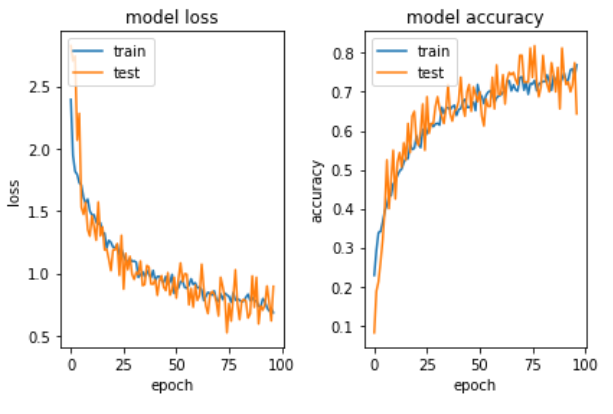
\includegraphics[width=250px]{sections/exp-1/images/model-2-acc.png}
    \captionof{figure}{Model 1 - Loss \& Accuracy}
\end{center}
